\begin{figure}
    \noindent
	\begin{minipage}[c]{.97\columnwidth}
        \centering
        \begin{lstlisting}[language={HTML5},frame=ltbr,aboveskip=1.1em,basicstyle={\linespread{1.0}\footnotesize\ttfamily},]
<form>
<section>
 <div><p>Name</p></div>
 <div><p>Business Email</p><span>free providers not accepted</span></div>
</section>
<input type="text" id="vr_9481">
<textarea id="bx_3978"></textarea>
<input type="text" id="vr_6588">
<div><p>Message</p></div>
<section>
 <div><p>Do you have an open ticket?</p></div>
 <div><p>How often should we email you?</p></div>
 <span>Yes</span><span>No</span>
</section>
<input type="radio" value="Y" id="op_y">
<input type="radio" value="N" id="op_n" checked>
<select id="frq"><option>daily</option>
 <option>weekly</option><option>monthly</option>
</select>
</form>
        \end{lstlisting}
    (a) Sample of the HTML markup
    \end{minipage} \hfill
	\begin{minipage}[c]{\columnwidth}
        \centering
        \fbox{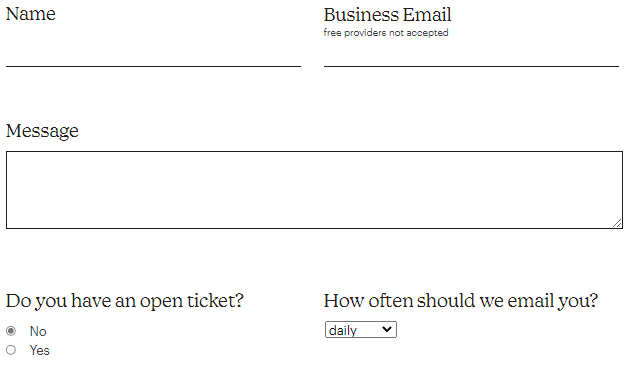
\includegraphics[width=\linewidth]{accessibility_repair/figures/motivating-example/rendered.png}}
        (b) Rendered form
    \end{minipage}
%	\begin{minipage}[c]{.98\columnwidth}
%	\centering \ \\
%	(a) Sample of the HTML markup
%	\end{minipage}
%	\begin{minipage}[c]{.98\columnwidth}
%	\centering \ \\
%	(b) Rendered form
%	\end{minipage}
	\ \\ \caption{An example of an inaccessible web form.}
    \label{fig:motivating-example}
  \end{figure}